%%
% Copyright (c) 2017 - 2019, Pascal Wagler;  
% Copyright (c) 2014 - 2019, John MacFarlane
% 
% All rights reserved.
% 
% Redistribution and use in source and binary forms, with or without 
% modification, are permitted provided that the following conditions 
% are met:
% 
% - Redistributions of source code must retain the above copyright 
% notice, this list of conditions and the following disclaimer.
% 
% - Redistributions in binary form must reproduce the above copyright 
% notice, this list of conditions and the following disclaimer in the 
% documentation and/or other materials provided with the distribution.
% 
% - Neither the name of John MacFarlane nor the names of other 
% contributors may be used to endorse or promote products derived 
% from this software without specific prior written permission.
% 
% THIS SOFTWARE IS PROVIDED BY THE COPYRIGHT HOLDERS AND CONTRIBUTORS 
% "AS IS" AND ANY EXPRESS OR IMPLIED WARRANTIES, INCLUDING, BUT NOT 
% LIMITED TO, THE IMPLIED WARRANTIES OF MERCHANTABILITY AND FITNESS 
% FOR A PARTICULAR PURPOSE ARE DISCLAIMED. IN NO EVENT SHALL THE 
% COPYRIGHT OWNER OR CONTRIBUTORS BE LIABLE FOR ANY DIRECT, INDIRECT, 
% INCIDENTAL, SPECIAL, EXEMPLARY, OR CONSEQUENTIAL DAMAGES (INCLUDING,
% BUT NOT LIMITED TO, PROCUREMENT OF SUBSTITUTE GOODS OR SERVICES; 
% LOSS OF USE, DATA, OR PROFITS; OR BUSINESS INTERRUPTION) HOWEVER 
% CAUSED AND ON ANY THEORY OF LIABILITY, WHETHER IN CONTRACT, STRICT 
% LIABILITY, OR TORT (INCLUDING NEGLIGENCE OR OTHERWISE) ARISING IN 
% ANY WAY OUT OF THE USE OF THIS SOFTWARE, EVEN IF ADVISED OF THE 
% POSSIBILITY OF SUCH DAMAGE.
%%

%%
% This is the Eisvogel pandoc LaTeX template.
%
% For usage information and examples visit the official GitHub page:
% https://github.com/Wandmalfarbe/pandoc-latex-template
%%

\PassOptionsToPackage{unicode=true}{hyperref} % options for packages loaded elsewhere
\PassOptionsToPackage{hyphens}{url}
\PassOptionsToPackage{dvipsnames,svgnames*,x11names*,table}{xcolor}
%
\documentclass[
  10pt,
  english,
  letterpaper,
,tablecaptionabove
]{scrartcl}
\usepackage{lmodern}
\usepackage{setspace}
\setstretch{1.2}
\usepackage{amssymb,amsmath}
\usepackage{ifxetex,ifluatex}
\ifnum 0\ifxetex 1\fi\ifluatex 1\fi=0 % if pdftex
  \usepackage[T1]{fontenc}
  \usepackage[utf8]{inputenc}
  \usepackage{textcomp} % provides euro and other symbols
\else % if luatex or xelatex
  \usepackage{unicode-math}
  \defaultfontfeatures{Scale=MatchLowercase}
  \defaultfontfeatures[\rmfamily]{Ligatures=TeX,Scale=1}
\fi
% use upquote if available, for straight quotes in verbatim environments
\IfFileExists{upquote.sty}{\usepackage{upquote}}{}
\IfFileExists{microtype.sty}{% use microtype if available
  \usepackage[]{microtype}
  \UseMicrotypeSet[protrusion]{basicmath} % disable protrusion for tt fonts
}{}
\makeatletter
\@ifundefined{KOMAClassName}{% if non-KOMA class
  \IfFileExists{parskip.sty}{%
    \usepackage{parskip}
  }{% else
    \setlength{\parindent}{0pt}
    \setlength{\parskip}{6pt plus 2pt minus 1pt}}
}{% if KOMA class
  \KOMAoptions{parskip=half}}
\makeatother
\usepackage{xcolor}
\definecolor{default-linkcolor}{HTML}{A50000}
\definecolor{default-filecolor}{HTML}{A50000}
\definecolor{default-citecolor}{HTML}{4077C0}
\definecolor{default-urlcolor}{HTML}{4077C0}
\IfFileExists{xurl.sty}{\usepackage{xurl}}{} % add URL line breaks if available
\IfFileExists{bookmark.sty}{\usepackage{bookmark}}{\usepackage{hyperref}}
\hypersetup{
  pdftitle={Red-Black Trees (Part 2)},
  pdfauthor={Connor Baker},
  pdfsubject={Red-Black Trees},
  pdfkeywords={Lecture, Red-Black, Self-Balancing Trees},
  pdfborder={0 0 0},
  breaklinks=true}
\urlstyle{same}  % don't use monospace font for urls
\usepackage[margin=2.5cm,includehead=true,includefoot=true,centering]{geometry}
\usepackage{listings}
\newcommand{\passthrough}[1]{#1}
\lstset{defaultdialect=[5.3]Lua}
\lstset{defaultdialect=[x86masm]Assembler}
\usepackage{longtable,booktabs}
% Allow footnotes in longtable head/foot
\IfFileExists{footnotehyper.sty}{\usepackage{footnotehyper}}{\usepackage{footnote}}
\makesavenoteenv{longtable}
\usepackage{graphicx,grffile}
\makeatletter
\def\maxwidth{\ifdim\Gin@nat@width>\linewidth\linewidth\else\Gin@nat@width\fi}
\def\maxheight{\ifdim\Gin@nat@height>\textheight\textheight\else\Gin@nat@height\fi}
\makeatother
% Scale images if necessary, so that they will not overflow the page
% margins by default, and it is still possible to overwrite the defaults
% using explicit options in \includegraphics[width, height, ...]{}
\setkeys{Gin}{width=\maxwidth,height=\maxheight,keepaspectratio}
\setlength{\emergencystretch}{3em}  % prevent overfull lines
\providecommand{\tightlist}{%
  \setlength{\itemsep}{0pt}\setlength{\parskip}{0pt}}
\setcounter{secnumdepth}{-\maxdimen} % remove section numbering
% Redefines (sub)paragraphs to behave more like sections
\ifx\paragraph\undefined\else
  \let\oldparagraph\paragraph
  \renewcommand{\paragraph}[1]{\oldparagraph{#1}\mbox{}}
\fi
\ifx\subparagraph\undefined\else
  \let\oldsubparagraph\subparagraph
  \renewcommand{\subparagraph}[1]{\oldsubparagraph{#1}\mbox{}}
\fi

% Make use of float-package and set default placement for figures to H
\usepackage{float}
\floatplacement{figure}{H}

\setcounter{page}{0}
\lstset{breaklines=true}
\lstset{postbreak=\raisebox{0ex}[0ex][0ex]{\ensuremath{\color{blue}\hookrightarrow\space}}}
\usepackage{datetime}
\settimeformat{ampmtime}
\usepackage{lastpage}
\ifnum 0\ifxetex 1\fi=0 % if pdftex or luatex
  \usepackage[shorthands=off,main=english]{babel}
\else % if xetex
    % See issue https://github.com/reutenauer/polyglossia/issues/127
  \renewcommand*\familydefault{\sfdefault}
    % load polyglossia as late as possible as it *could* call bidi if RTL lang (e.g. Hebrew or Arabic)
  \usepackage{polyglossia}
  \setmainlanguage[]{english}
\fi

\title{Red-Black Trees (Part 2)}
\usepackage{etoolbox}
\makeatletter
\providecommand{\subtitle}[1]{% add subtitle to \maketitle
  \apptocmd{\@title}{\par {\large #1 \par}}{}{}
}
\makeatother
\subtitle{Red-black trees, more rotation cases, insertion, and complexity}
\author{Connor Baker}
\date{2019-04-18, Compiled on \today~at \currenttime}





%%
%% added
%%

%
% language specification
%
% If no language is specified, use English as the default main document language.
%


%
% for the background color of the title page
%
\usepackage{pagecolor}
\usepackage{afterpage}

%
% TOC depth and 
% section numbering depth
%
\setcounter{tocdepth}{3}

%
% break urls
%
\PassOptionsToPackage{hyphens}{url}

%
% When using babel or polyglossia with biblatex, loading csquotes is recommended 
% to ensure that quoted texts are typeset according to the rules of your main language.
%
\usepackage{csquotes}

%
% captions
%
\definecolor{caption-color}{HTML}{777777}
\usepackage[font={stretch=1.2}, textfont={color=caption-color}, position=top, skip=4mm, labelfont=bf, singlelinecheck=false, justification=raggedright]{caption}
\setcapindent{0em}

%
% blockquote
%
\definecolor{blockquote-border}{RGB}{221,221,221}
\definecolor{blockquote-text}{RGB}{119,119,119}
\usepackage{mdframed}
\newmdenv[rightline=false,bottomline=false,topline=false,linewidth=3pt,linecolor=blockquote-border,skipabove=\parskip]{customblockquote}
\renewenvironment{quote}{\begin{customblockquote}\list{}{\rightmargin=0em\leftmargin=0em}%
\item\relax\color{blockquote-text}\ignorespaces}{\unskip\unskip\endlist\end{customblockquote}}

%
% Source Sans Pro as the de­fault font fam­ily
% Source Code Pro for monospace text
%
% 'default' option sets the default 
% font family to Source Sans Pro, not \sfdefault.
%
\usepackage[default]{sourcesanspro}
\usepackage{sourcecodepro}

% XeLaTeX specific adjustments for straight quotes: https://tex.stackexchange.com/a/354887
% This issue is already fixed (see https://github.com/silkeh/latex-sourcecodepro/pull/5) but the 
% fix is still unreleased.
% TODO: Remove this workaround when the new version of sourcecodepro is released on CTAN.
\ifxetex
\makeatletter
\defaultfontfeatures[\ttfamily]
  { Numbers   = \sourcecodepro@figurestyle,
    Scale     = \SourceCodePro@scale,
    Extension = .otf }
\setmonofont
  [ UprightFont    = *-\sourcecodepro@regstyle,
    ItalicFont     = *-\sourcecodepro@regstyle It,
    BoldFont       = *-\sourcecodepro@boldstyle,
    BoldItalicFont = *-\sourcecodepro@boldstyle It ]
  {SourceCodePro}
\makeatother
\fi

%
% heading color
%
\definecolor{heading-color}{RGB}{40,40,40}
\addtokomafont{section}{\color{heading-color}}
% When using the classes report, scrreprt, book, 
% scrbook or memoir, uncomment the following line.
%\addtokomafont{chapter}{\color{heading-color}}

%
% variables for title and author
%
\usepackage{titling}
\title{Red-Black Trees (Part 2)}
\author{Connor Baker}

%
% tables
%

\definecolor{table-row-color}{HTML}{F5F5F5}
\definecolor{table-rule-color}{HTML}{999999}

%\arrayrulecolor{black!40}
\arrayrulecolor{table-rule-color}     % color of \toprule, \midrule, \bottomrule
\setlength\heavyrulewidth{0.3ex}      % thickness of \toprule, \bottomrule
\renewcommand{\arraystretch}{1.3}     % spacing (padding)

% Reset rownum counter so that each table
% starts with the same row colors.
% https://tex.stackexchange.com/questions/170637/restarting-rowcolors
\let\oldlongtable\longtable
\let\endoldlongtable\endlongtable
\renewenvironment{longtable}{
\rowcolors{3}{}{table-row-color!100}  % row color
\oldlongtable} {
\endoldlongtable
\global\rownum=0\relax}

% Unfortunately the colored cells extend beyond the edge of the 
% table because pandoc uses @-expressions (@{}) like so: 
%
% \begin{longtable}[]{@{}ll@{}}
% \end{longtable}
%
% https://en.wikibooks.org/wiki/LaTeX/Tables#.40-expressions

%
% remove paragraph indention
%
\setlength{\parindent}{0pt}
\setlength{\parskip}{6pt plus 2pt minus 1pt}
\setlength{\emergencystretch}{3em}  % prevent overfull lines

%
%
% Listings
%
%


%
% listing colors
%
\definecolor{listing-background}{HTML}{F7F7F7}
\definecolor{listing-rule}{HTML}{B3B2B3}
\definecolor{listing-numbers}{HTML}{B3B2B3}
\definecolor{listing-text-color}{HTML}{000000}
\definecolor{listing-keyword}{HTML}{435489}
\definecolor{listing-identifier}{HTML}{435489}
\definecolor{listing-string}{HTML}{00999A}
\definecolor{listing-comment}{HTML}{8E8E8E}
\definecolor{listing-javadoc-comment}{HTML}{006CA9}

\lstdefinestyle{eisvogel_listing_style}{
  language         = java,
  numbers          = left,
  xleftmargin      = 2.7em,
  framexleftmargin = 2.5em,
  backgroundcolor  = \color{listing-background},
  basicstyle       = \color{listing-text-color}\small\ttfamily{}\linespread{1.15}, % print whole listing small
  breaklines       = true,
  frame            = single,
  framesep         = 0.19em,
  rulecolor        = \color{listing-rule},
  frameround       = ffff,
  tabsize          = 4,
  numberstyle      = \color{listing-numbers},
  aboveskip        = -0.7em,
  belowskip        = 0.1em,
  abovecaptionskip = 0em,
  belowcaptionskip = 1em,
  keywordstyle     = \color{listing-keyword}\bfseries,
  classoffset      = 0,
  sensitive        = true,
  identifierstyle  = \color{listing-identifier},
  commentstyle     = \color{listing-comment},
  morecomment      = [s][\color{listing-javadoc-comment}]{/**}{*/},
  stringstyle      = \color{listing-string},
  showstringspaces = false,
  escapeinside     = {/*@}{@*/}, % Allow LaTeX inside these special comments
  literate         =
  {á}{{\'a}}1 {é}{{\'e}}1 {í}{{\'i}}1 {ó}{{\'o}}1 {ú}{{\'u}}1
  {Á}{{\'A}}1 {É}{{\'E}}1 {Í}{{\'I}}1 {Ó}{{\'O}}1 {Ú}{{\'U}}1
  {à}{{\`a}}1 {è}{{\'e}}1 {ì}{{\`i}}1 {ò}{{\`o}}1 {ù}{{\`u}}1
  {À}{{\`A}}1 {È}{{\'E}}1 {Ì}{{\`I}}1 {Ò}{{\`O}}1 {Ù}{{\`U}}1
  {ä}{{\"a}}1 {ë}{{\"e}}1 {ï}{{\"i}}1 {ö}{{\"o}}1 {ü}{{\"u}}1
  {Ä}{{\"A}}1 {Ë}{{\"E}}1 {Ï}{{\"I}}1 {Ö}{{\"O}}1 {Ü}{{\"U}}1
  {â}{{\^a}}1 {ê}{{\^e}}1 {î}{{\^i}}1 {ô}{{\^o}}1 {û}{{\^u}}1
  {Â}{{\^A}}1 {Ê}{{\^E}}1 {Î}{{\^I}}1 {Ô}{{\^O}}1 {Û}{{\^U}}1
  {œ}{{\oe}}1 {Œ}{{\OE}}1 {æ}{{\ae}}1 {Æ}{{\AE}}1 {ß}{{\ss}}1
  {ç}{{\c c}}1 {Ç}{{\c C}}1 {ø}{{\o}}1 {å}{{\r a}}1 {Å}{{\r A}}1
  {€}{{\EUR}}1 {£}{{\pounds}}1 {«}{{\guillemotleft}}1
  {»}{{\guillemotright}}1 {ñ}{{\~n}}1 {Ñ}{{\~N}}1 {¿}{{?`}}1
  {…}{{\ldots}}1 {≥}{{>=}}1 {≤}{{<=}}1 {„}{{\glqq}}1 {“}{{\grqq}}1
  {”}{{''}}1
}
\lstset{style=eisvogel_listing_style}

\lstdefinelanguage{XML}{
  morestring      = [b]",
  moredelim       = [s][\bfseries\color{listing-keyword}]{<}{\ },
  moredelim       = [s][\bfseries\color{listing-keyword}]{</}{>},
  moredelim       = [l][\bfseries\color{listing-keyword}]{/>},
  moredelim       = [l][\bfseries\color{listing-keyword}]{>},
  morecomment     = [s]{<?}{?>},
  morecomment     = [s]{<!--}{-->},
  commentstyle    = \color{listing-comment},
  stringstyle     = \color{listing-string},
  identifierstyle = \color{listing-identifier}
}

%
% header and footer
%
\usepackage{fancyhdr}

\fancypagestyle{eisvogel-header-footer}{
  \fancyhead{}
  \fancyfoot{}
  \lhead[2019-04-18]{Red-Black Trees (Part 2)}
  \chead[]{}
  \rhead[Red-Black Trees (Part 2)]{2019-04-18}
  \lfoot[\thepage~of \pageref{LastPage}]{Connor Baker}
  \cfoot[]{}
  \rfoot[Connor Baker]{\thepage~of \pageref{LastPage}}
  \renewcommand{\headrulewidth}{0.4pt}
  \renewcommand{\footrulewidth}{0.4pt}
}
\pagestyle{eisvogel-header-footer}

%%
%% end added
%%

\begin{document}

%%
%% begin titlepage
%%

\begin{titlepage}
\newgeometry{left=6cm}
\definecolor{titlepage-color}{HTML}{FFFFFF}
\newpagecolor{titlepage-color}\afterpage{\restorepagecolor}
\newcommand{\colorRule}[3][black]{\textcolor[HTML]{#1}{\rule{#2}{#3}}}
\begin{flushleft}
\noindent
\\[-1em]
\color[HTML]{0d47a1}
\makebox[0pt][l]{\colorRule[0d47a1]{1.3\textwidth}{2pt}}
\par
\noindent

{ \setstretch{1.4}
\vfill
\noindent {\huge \textbf{\textsf{Red-Black Trees (Part 2)}}}
\vskip 1em
{\Large \textsf{Red-black trees, more rotation cases, insertion, and complexity}}
\vskip 2em
\noindent
{\Large \textsf{Connor Baker}
\vfill
}


\textsf{2019-04-18, Compiled on \today~at \currenttime}}
\end{flushleft}
\end{titlepage}
\restoregeometry

%%
%% end titlepage
%%



\hypertarget{red-black-trees-part-2}{%
\section{Red-Black Trees (Part 2)}\label{red-black-trees-part-2}}

\hypertarget{review}{%
\subsection{Review}\label{review}}

\begin{itemize}
\tightlist
\item
  Color properties
\item
  Insertion: add new values as a red leaf

  \begin{itemize}
  \tightlist
  \item
    Black parent
  \item
    Red parent and red uncle

    \begin{itemize}
    \tightlist
    \item
      Recoloring
    \end{itemize}
  \item
    Red parent and black uncle

    \begin{itemize}
    \tightlist
    \item
      Rotation and recoloring
    \end{itemize}
  \end{itemize}
\end{itemize}

\hypertarget{rotation-general-cases}{%
\subsection{Rotation General Cases}\label{rotation-general-cases}}

\begin{itemize}
\tightlist
\item
  The new node is red, the parent is red, and the uncle is black

  \begin{itemize}
  \tightlist
  \item
    Note: more black on the uncle's side of the tree
  \end{itemize}
\item
  Step 1: perform a rotation at the parent \emph{if needed}

  \begin{itemize}
  \tightlist
  \item
    \textbf{When do we do this? Why?}
  \end{itemize}
\end{itemize}

\begin{figure}
\centering
\includegraphics[width=0.75\textwidth,height=\textheight]{images/1.png}
\caption{Step 1}
\end{figure}

\begin{itemize}
\tightlist
\item
  Step 2: perform a rotation at the grandparent
\item
  Step 3: swap the old parent and the grandparent's colors
\end{itemize}

\begin{figure}
\centering
\includegraphics[width=0.75\textwidth,height=\textheight]{images/2.png}
\caption{Steps 2 and 3}
\end{figure}

\begin{itemize}
\tightlist
\item
  We could potentially need an additional step in certain cases

  \begin{itemize}
  \tightlist
  \item
    Consider the case where we need to use a left-rotation with the
    newly inserted node
  \end{itemize}
\end{itemize}

\begin{figure}
\centering
\includegraphics[width=0.75\textwidth,height=\textheight]{images/3.png}
\caption{An extra rotation may be needed}
\end{figure}

\hypertarget{problems-with-red-subtree-roots}{%
\subsection{Problems with Red Subtree
Roots}\label{problems-with-red-subtree-roots}}

\begin{itemize}
\tightlist
\item
  Remaining issue: if a recolor makes a subtree root red, then we may
  have create two consecutive red nodes!
\item
  Strategy one: detect and travel back up to perform additional fixes

  \begin{itemize}
  \tightlist
  \item
    We can always change the root to black for a final fix
  \item
    We do however have to go up to fix the nodes with rotation or
    recoloring
  \end{itemize}
\end{itemize}

\hypertarget{example}{%
\subsection{Example}\label{example}}

\begin{itemize}
\tightlist
\item
  Suppose we want to insert \(45\) into the following red-black tree.
\end{itemize}

\begin{figure}
\centering
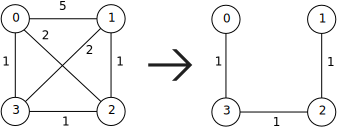
\includegraphics[width=1\textwidth,height=\textheight]{images/4.png}
\caption{A red-black tree}
\end{figure}

\begin{itemize}
\tightlist
\item
  Trying to do so would land us with a red-red combo, where the uncle is
  also red

  \begin{itemize}
  \tightlist
  \item
    As such, we'd need to recolor them
  \item
    This requires (possibly) more rotations and recoloring up the tree
  \end{itemize}
\end{itemize}

\hypertarget{top-down-approach}{%
\subsection{Top-Down Approach}\label{top-down-approach}}

\begin{itemize}
\tightlist
\item
  Strategy two: down only (top-down insertion)

  \begin{itemize}
  \tightlist
  \item
    In a single downwards pass, recolor and rotate to ensure that the
    insertion will succeed without us having to walk back up the tree to
    fix it afterwards
  \end{itemize}
\item
  What might cause trouble for us so that we need to go back up the tree
  to fix it?

  \begin{itemize}
  \tightlist
  \item
    Black parent: easy, no issue there
  \item
    Red parent

    \begin{itemize}
    \tightlist
    \item
      \textbf{Black uncle?}
    \item
      \textbf{Red uncle?}
    \end{itemize}
  \end{itemize}
\end{itemize}

\hypertarget{black-uncle}{%
\subsection{Black Uncle}\label{black-uncle}}

\begin{figure}
\centering
\includegraphics[width=1\textwidth,height=\textheight]{images/5.png}
\caption{Cases with a black uncle}
\end{figure}

\hypertarget{red-uncle}{%
\subsection{Red Uncle}\label{red-uncle}}

\begin{figure}
\centering
\includegraphics[width=1\textwidth,height=\textheight]{images/6.png}
\caption{Case with a red uncle}
\end{figure}

\hypertarget{top-down-insertion}{%
\subsection{Top-Down Insertion}\label{top-down-insertion}}

\begin{itemize}
\tightlist
\item
  The fix: guarantee that the red parent does not have a red sibling

  \begin{itemize}
  \tightlist
  \item
    One the way down we need to check the (black) node
    \passthrough{\lstinline!n!}
  \item
    If both children are red, chang ethe children to black and change
    \passthrough{\lstinline!n!} to red

    \begin{itemize}
    \tightlist
    \item
      \textbf{What if \passthrough{\lstinline!n!} is the root?}
    \end{itemize}
  \item
    If the parent of \passthrough{\lstinline!n!} is red, use a
    single/double rotation and recoloring to fix, then continue down the
    tree

    \begin{itemize}
    \tightlist
    \item
      \textbf{Can \passthrough{\lstinline!n!} have a red uncle?}
    \end{itemize}
  \item
    Ensure that after the red inserction, we only need to perform local
    adjustments

    \begin{itemize}
    \tightlist
    \item
      There is no percolating back up
    \end{itemize}
  \end{itemize}
\end{itemize}

\hypertarget{example-continued}{%
\subsection{Example (Continued)}\label{example-continued}}

\begin{itemize}
\tightlist
\item
  Back to our previous example of trying to insert \(45\) into a
  red-black tree:
\end{itemize}

\begin{figure}
\centering
\includegraphics[width=1\textwidth,height=\textheight]{images/7.png}
\caption{Top-down insertion with a red-black tree}
\end{figure}

\hypertarget{complexity}{%
\subsection{Complexity}\label{complexity}}

\begin{itemize}
\tightlist
\item
  A red-black tree which contains \(n\) nodes has a height of
  \(O(\log(n))\)

  \begin{itemize}
  \tightlist
  \item
    A detailed proof is available on
    \href{http://en.wikipedia.org/wiki/Red\%E2\%80\%93black_tree}{Wikipedia's
    Red-Black Tree page}
  \end{itemize}
\item
  Notes
\item
  The black height (\passthrough{\lstinline!bh!}) of a node
  \passthrough{\lstinline!m!} counts the number of black nodes from
  \passthrough{\lstinline!n!} to a \passthrough{\lstinline!null!} link
  (not counting \passthrough{\lstinline!t!} if
  \passthrough{\lstinline!t!} is black)

  \begin{itemize}
  \tightlist
  \item
    Given \passthrough{\lstinline!bh(t)!}, the shortest path from
    \passthrough{\lstinline!n!} to any \passthrough{\lstinline!null!}
    link has \passthrough{\lstinline!bh(t)!} edges: all of which are
    black nodes
  \item
    Given \passthrough{\lstinline!bh(t)!}, the longet path from
    \passthrough{\lstinline!t!} to any \passthrough{\lstinline!null!}
    link has \passthrough{\lstinline!2 * bh(t)!} edges: the nodes
    alternate between red and black
  \item
    \passthrough{\lstinline!bh(t) >= h(t) / 2!}, where
    \passthrough{\lstinline!h(t)!} is the height of
    \passthrough{\lstinline!t!} where `h(null) = 0
  \item
    The height of a nod \passthrough{\lstinline!t!}:
    \passthrough{\lstinline!h(t)!} is bounded above by
    \passthrough{\lstinline!2 * bh(t)!}
  \item
    Number of nodes rooted at \passthrough{\lstinline!t!}: bounded below
    by \passthrough{\lstinline!2^bh(t) - 1 <= N!}

    \begin{itemize}
    \tightlist
    \item
      Proof by induction on \passthrough{\lstinline!height!} and
      \passthrough{\lstinline!bh!}
    \end{itemize}
  \item
    \passthrough{\lstinline!h(t) <= 2 log(2, N + 1)!} where
    \passthrough{\lstinline!N!} is the size of the tree
  \end{itemize}
\end{itemize}

\hypertarget{avl-trees-vs.-red-black-trees}{%
\subsection{AVL Trees vs.~Red-Black
Trees}\label{avl-trees-vs.-red-black-trees}}

\hypertarget{avl-trees}{%
\subsubsection{AVL Trees}\label{avl-trees}}

\begin{itemize}
\tightlist
\item
  Pros

  \begin{itemize}
  \tightlist
  \item
    Simple(r) to implement
  \item
    Faster lookup (maintains optimal height)
  \end{itemize}
\item
  Cons

  \begin{itemize}
  \tightlist
  \item
    Slower to insert or delete (because it must maintain optimall
    height)
  \item
    Simple implementation is recursive and relies on down-up toslutions
  \end{itemize}
\end{itemize}

\hypertarget{red-black-trees}{%
\subsubsection{Red-Black Trees}\label{red-black-trees}}

\begin{itemize}
\tightlist
\item
  Pros

  \begin{itemize}
  \tightlist
  \item
    Faster insert/delete (doesn't have to maintain optimal height)
  \item
    Implementation tricks can do down-only insertion and deletion
  \end{itemize}
\item
  Cons

  \begin{itemize}
  \tightlist
  \item
    Complex algorithm
  \item
    Slower lookup (doesn't have optimal height)
  \item
    Implementation is complicated
  \end{itemize}
\end{itemize}

\hypertarget{balanced-bst-benefits}{%
\subsection{Balanced BST Benefits}\label{balanced-bst-benefits}}

\begin{itemize}
\tightlist
\item
  Keep data in order
\item
  Provided guarantee \(O(\log(N))\) find/add/remove
\item
  Reproduce sorted order via an in-order traversal
\item
  Reproduce sorted slices of data

  \begin{itemize}
  \tightlist
  \item
    Locate a record in \(O(\log(N))\) time
  \item
    In-order traversa from that record
  \end{itemize}
\end{itemize}

\hypertarget{sets-and-maps-review}{%
\subsection{Sets and Maps Review}\label{sets-and-maps-review}}

\begin{itemize}
\tightlist
\item
  Closely related data structures

  \begin{itemize}
  \tightlist
  \item
    A collection of (usually distinct) values
  \item
    Supports efficient look-up

    \begin{itemize}
    \tightlist
    \item
      Do we have this value or not?
    \item
      Is there a value associated with this key\textgreater{}
    \end{itemize}
  \end{itemize}
\item
  Conventions:

  \begin{itemize}
  \tightlist
  \item
    Do not allow keys to be null
  \item
    Do not allow duplicate values for a key

    \begin{itemize}
    \tightlist
    \item
      \passthrough{\lstinline!put(key1, val1)!} followed by
      \passthrough{\lstinline!put(key1, val2)!} sees
      \passthrough{\lstinline!val2!} overwrite
      \passthrough{\lstinline!val1!}
    \end{itemize}
  \item
    Iteration is allowed on the keys

    \begin{itemize}
    \tightlist
    \item
      We can the use the key to get the associated value
    \end{itemize}
  \end{itemize}
\end{itemize}

\hypertarget{maps-and-sets-implementations}{%
\subsection{Maps and Sets
Implementations}\label{maps-and-sets-implementations}}

\begin{itemize}
\tightlist
\item
  Main concern: can we efficiently handle a large number of
  \passthrough{\lstinline!get!} operations after a large number of
  \passthrough{\lstinline!put!} or \passthrough{\lstinline!get!}
  operations?
\item
  Naive implementations

  \begin{itemize}
  \tightlist
  \item
    Unordered linked list
  \item
    Ordered array
  \end{itemize}
\item
  Trees

  \begin{itemize}
  \tightlist
  \item
    Binary search trees
  \item
    Balanced binary search trees (AVL, Red-Black, AA)
  \end{itemize}
\item
  Hash tables
\end{itemize}

\hypertarget{maps-and-sets-big-o}{%
\subsection{\texorpdfstring{Maps and Sets
Big-\(O\)}{Maps and Sets Big-O}}\label{maps-and-sets-big-o}}

\begin{longtable}[]{ccccccc}
\toprule
Implementation & Worst Case & Worst Case & Average Case & Average Case &
Ordered & Remarks\tabularnewline
\midrule
\endhead
& Search & Insert & Search & Insert & &\tabularnewline
Unordered List & \(O(n)\) & \(O(n)^1\) & \(O(n)\) & \(O(n)^1\) & no
&\tabularnewline
Ordered List & \(O(\log(n))\) & \(O(n)\) & \(O(\log(n))\) & \(O(n)\) &
yes &\tabularnewline
HT Chaining & \(O(n)\) & \(O(n)\) & \(O(n/m)\) & \(O(n/m)\) & no & often
used\(^2\)\tabularnewline
HT Probing & \(O(n)\) & \(O(n)\) & \(O(1)\) & \(O(1)\) & no
&\tabularnewline
BSTs & \(O(n)\) & \(O(n)\) & \(O(\log(n))\) & \(O(\log(n))\) & yes &
easy\tabularnewline
AVLs & \(O(\log(n))\) & \(O(\log(n))\) & \(O(\log(n))\) & \(O(\log(n))\)
& yes & easy\tabularnewline
Red-Black Trees & \(O(\log(n))\) & \(O(\log(n))\) & \(O(\log(n))\) &
\(O(\log(n))\) & yes & often used\(^2\)\tabularnewline
\bottomrule
\end{longtable}

\begin{itemize}
\tightlist
\item
  \(n\): number of values
\item
  \(m\): number of entries
\item
  \(^1\): \(O(n)\) to check for duplicates, \(O(1)\) if this is not
  needed for some reason
\item
  \(^2\): Good constants and relatively easy to implement; used in many
  libraries
\end{itemize}

\hypertarget{next-lecture}{%
\subsection{Next Lecture}\label{next-lecture}}

\begin{itemize}
\tightlist
\item
  Disjoint sets: union/find
\item
  Reading: Chapter 24
\end{itemize}

\end{document}
